%****************************************************
%	CHAPTER 1 - INTRODUCTION
%****************************************************
\chapter{Introduction}
\label{ch:ch1}
%====================================================
\section{Background to investigation}
\label{sec:ch1.section1}

Antarctica plays host to ocean-atmospheric processes, which are significant drivers of global climate. These interactions are strongly influenced by sea ice coverage and extent, which acts as a boundary layer between the atmosphere and ocean \cite{parkinson2004southern}. Sea ice reflects incoming solar radiation which, otherwise, would be absorbed by the ocean thereby influencing ocean temperature and salinity \cite{parkinson2004southern}. Additionally, sea ice expanse  has been shown to insulate the ocean and reduce evaporation while regulating heat flux, and gaseous exchange \cite{deconto2003rapid} thereby providing a stable habitat for the diverse ecosystem that inhabits the region \cite{arrigo2004large} (see figure \ref{fig:AntaDiag}). Sea ice provides a damping effect on oceanic kinetic energy as it regulates the mass and movement of waves around the Southern Ocean \cite{parkinson2004southern,roach2020antarctic}. Sea ice coverage is fundamental to preserving a stable ocean environment as well as providing protection from extreme, weather conditions that affect the region \cite{vichi2019effects}. High winds, cyclone frequency and prominent wave activity perturbs the ice preventing it from congealing. The result is a region of semi-consolidated ice masses known as the Marginal Ice Zone (MIZ) \cite{vichi2019effects}.

Sea ice formation in the Southern Ocean begins when the surface layer of the ocean congeals causing ice crystals to form. These crystals combine to form frazil ice; the concentration of which increases as the heat from the ocean is removed by the atmosphere \cite{arrigo2004large}. As the wind and wave activity begin to calm, the frazil ice combines into grease ice, which grows into pancake ice floes \cite{arrigo2004large}. This growth period is known as "freeze-up" and forms the first stages of the sea ice life cycle \cite{barber2005microwave}. Additionally, Strong winds in the Marginal Ice Zones cause the floes to drift over long distances \cite{alberello2019drift}. These winds, coupled with high ice floe density result in collisions between ice floes causing them to break apart \cite{STEER2008933} resulting in brash ice \cite{icedefinition1992}.  During the winter months, newly formed ice grows a layer of snow \cite{barber2005microwave} and is termed "first year ice" \footnote{First year ice is newly consolidated ice that has been growing for less than one winter's growth period \cite{icedefinition1992}}, brine is present between the ice fragments and the layer of snow is affected by the level of precipitation \cite{barber2005microwave}.\par

\begin{figure}[H]
    \centering
    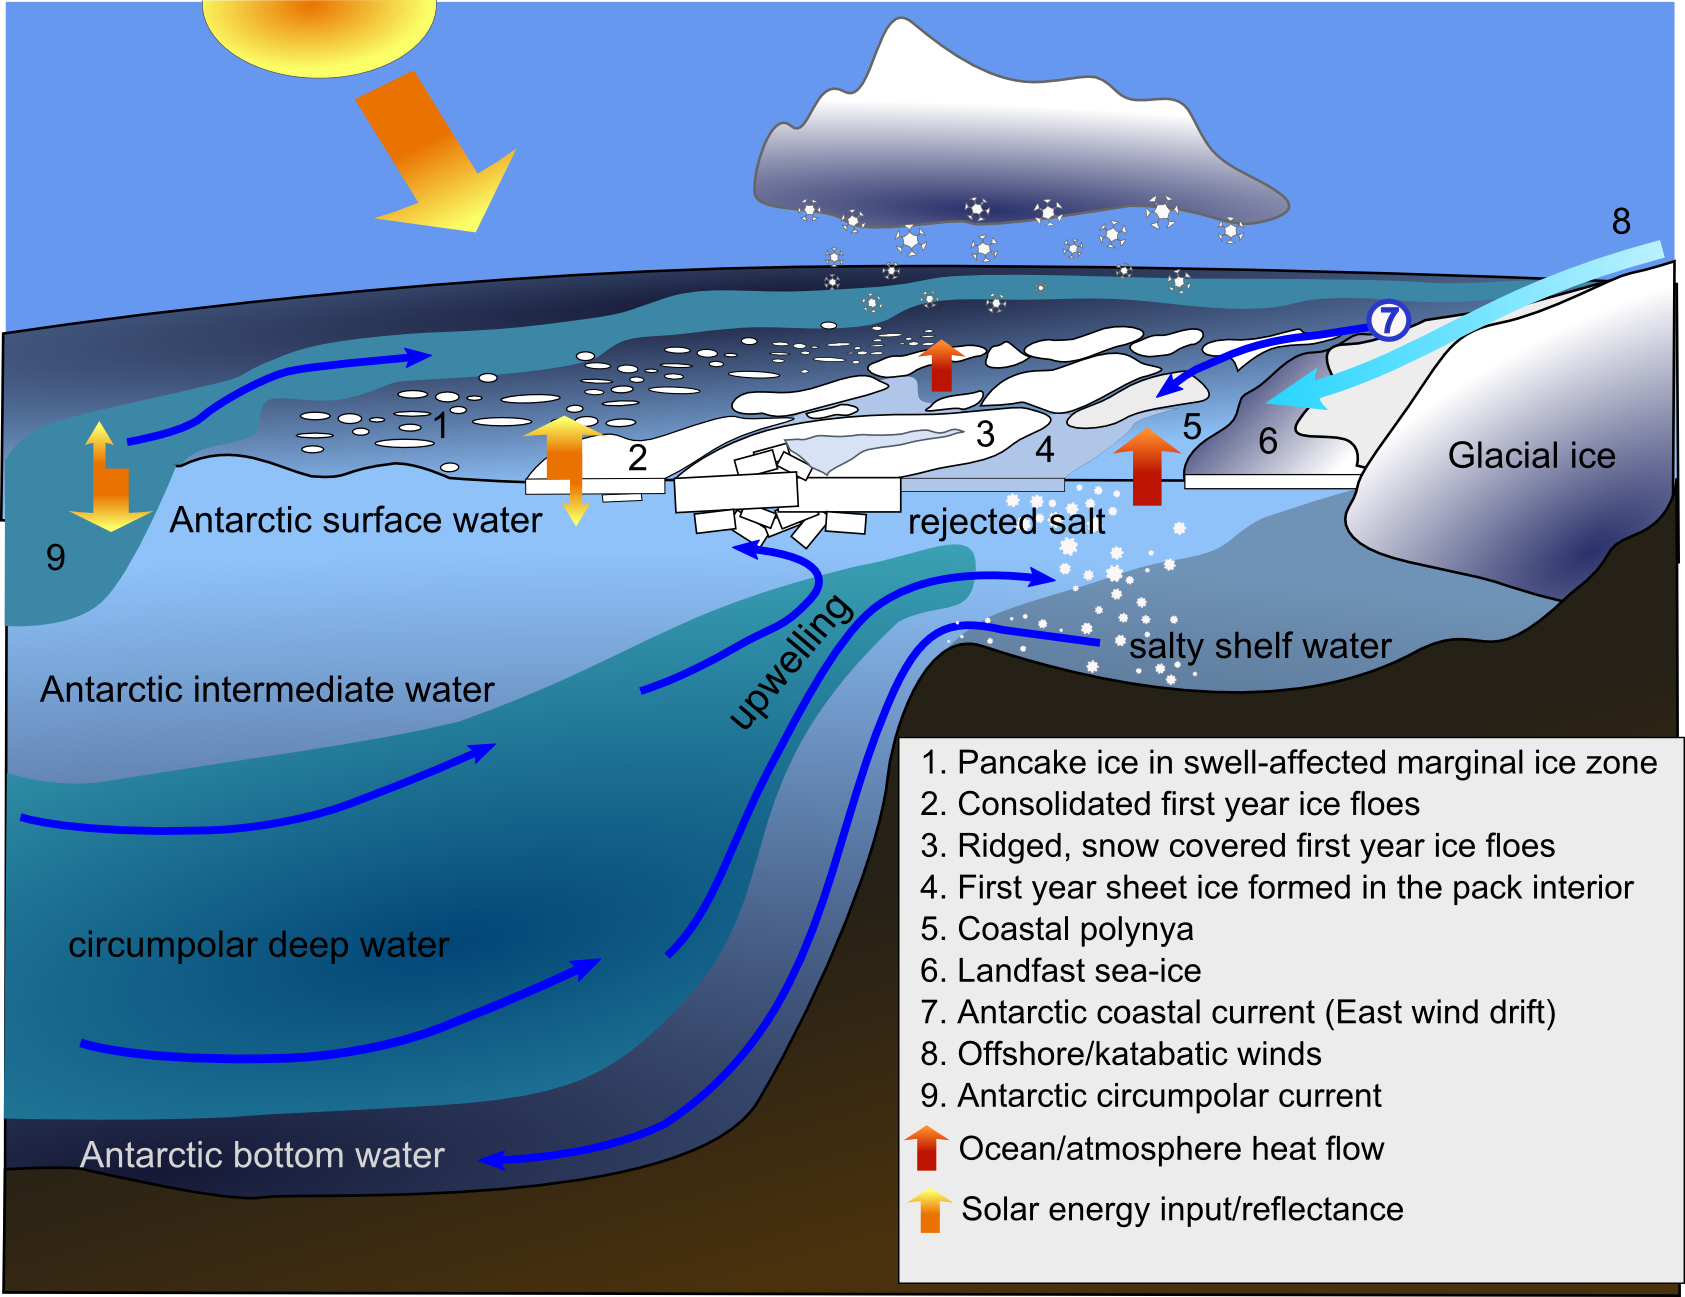
\includegraphics[width = 6cm,height=6cm]{AntDiag.png}
    \caption{Diagram showing the expanse of sea ice in the Southern Ocean. Packed ice forms closer to the continent in calmer conditions while strong oceanic currents,winds wave action and extreme temperatures result in the formation of semi-consolidated ice in the marginal ice zone (1 - 5). Here, ice formation is highly seasonal expanding to a maximum in winter and retreating to a minimum in summer. Sea ice acts as a boundary layer influencing heat and gaseous  exchange between the atmosphere and ocean. Figure taken from \textcite{Antseaice}}
    \label{fig:AntaDiag}
\end{figure}



Finally, the seasonal cycle closes with three phases of melting. Early melt marks the transitional period  where moisture is continuously present in snow cover on the sea ice \cite{barber2005microwave}. The level of moisture in the snow increases through "melt-onset" brought on by the transition from summer to winter and increasing ocean/atmospheric temperatures \cite{barber2005microwave}. Eventually, the snow and ice surface begin to melt rapidly during the "advanced melt" phase resulting in complete desalination of the ice floes followed by the breaking up of the sea ice sheets \cite{barber2005microwave}. 

The result of these processes is a region of semi-consolidated ice, which extends an estimated 19 million $\text{km}^2$ from the Antarctic continent \cite{MAKSYM2012seaiceextent}. These ice floes increase in size through gradual heating, fusing the floes into packed ice \cite{arrigo2004large}. Sea ice concentration in the MIZ is highly variable covering a range of 15\% to 85\% of total ice concentration from summer to winter respectively \cite{alberello2019drift}. The variability of the MIZ, coupled with the strong storms and weather patterns, drive the strongest atmospheric-ocean-sea ice interactions in the region. \textcite{alberello2019drift} further highlight that knowledge of MIZ sea ice dynamics is required to model the response to storms as well as predict the regional response to changes in climate.

\begin{figure}[H]
    \centering
   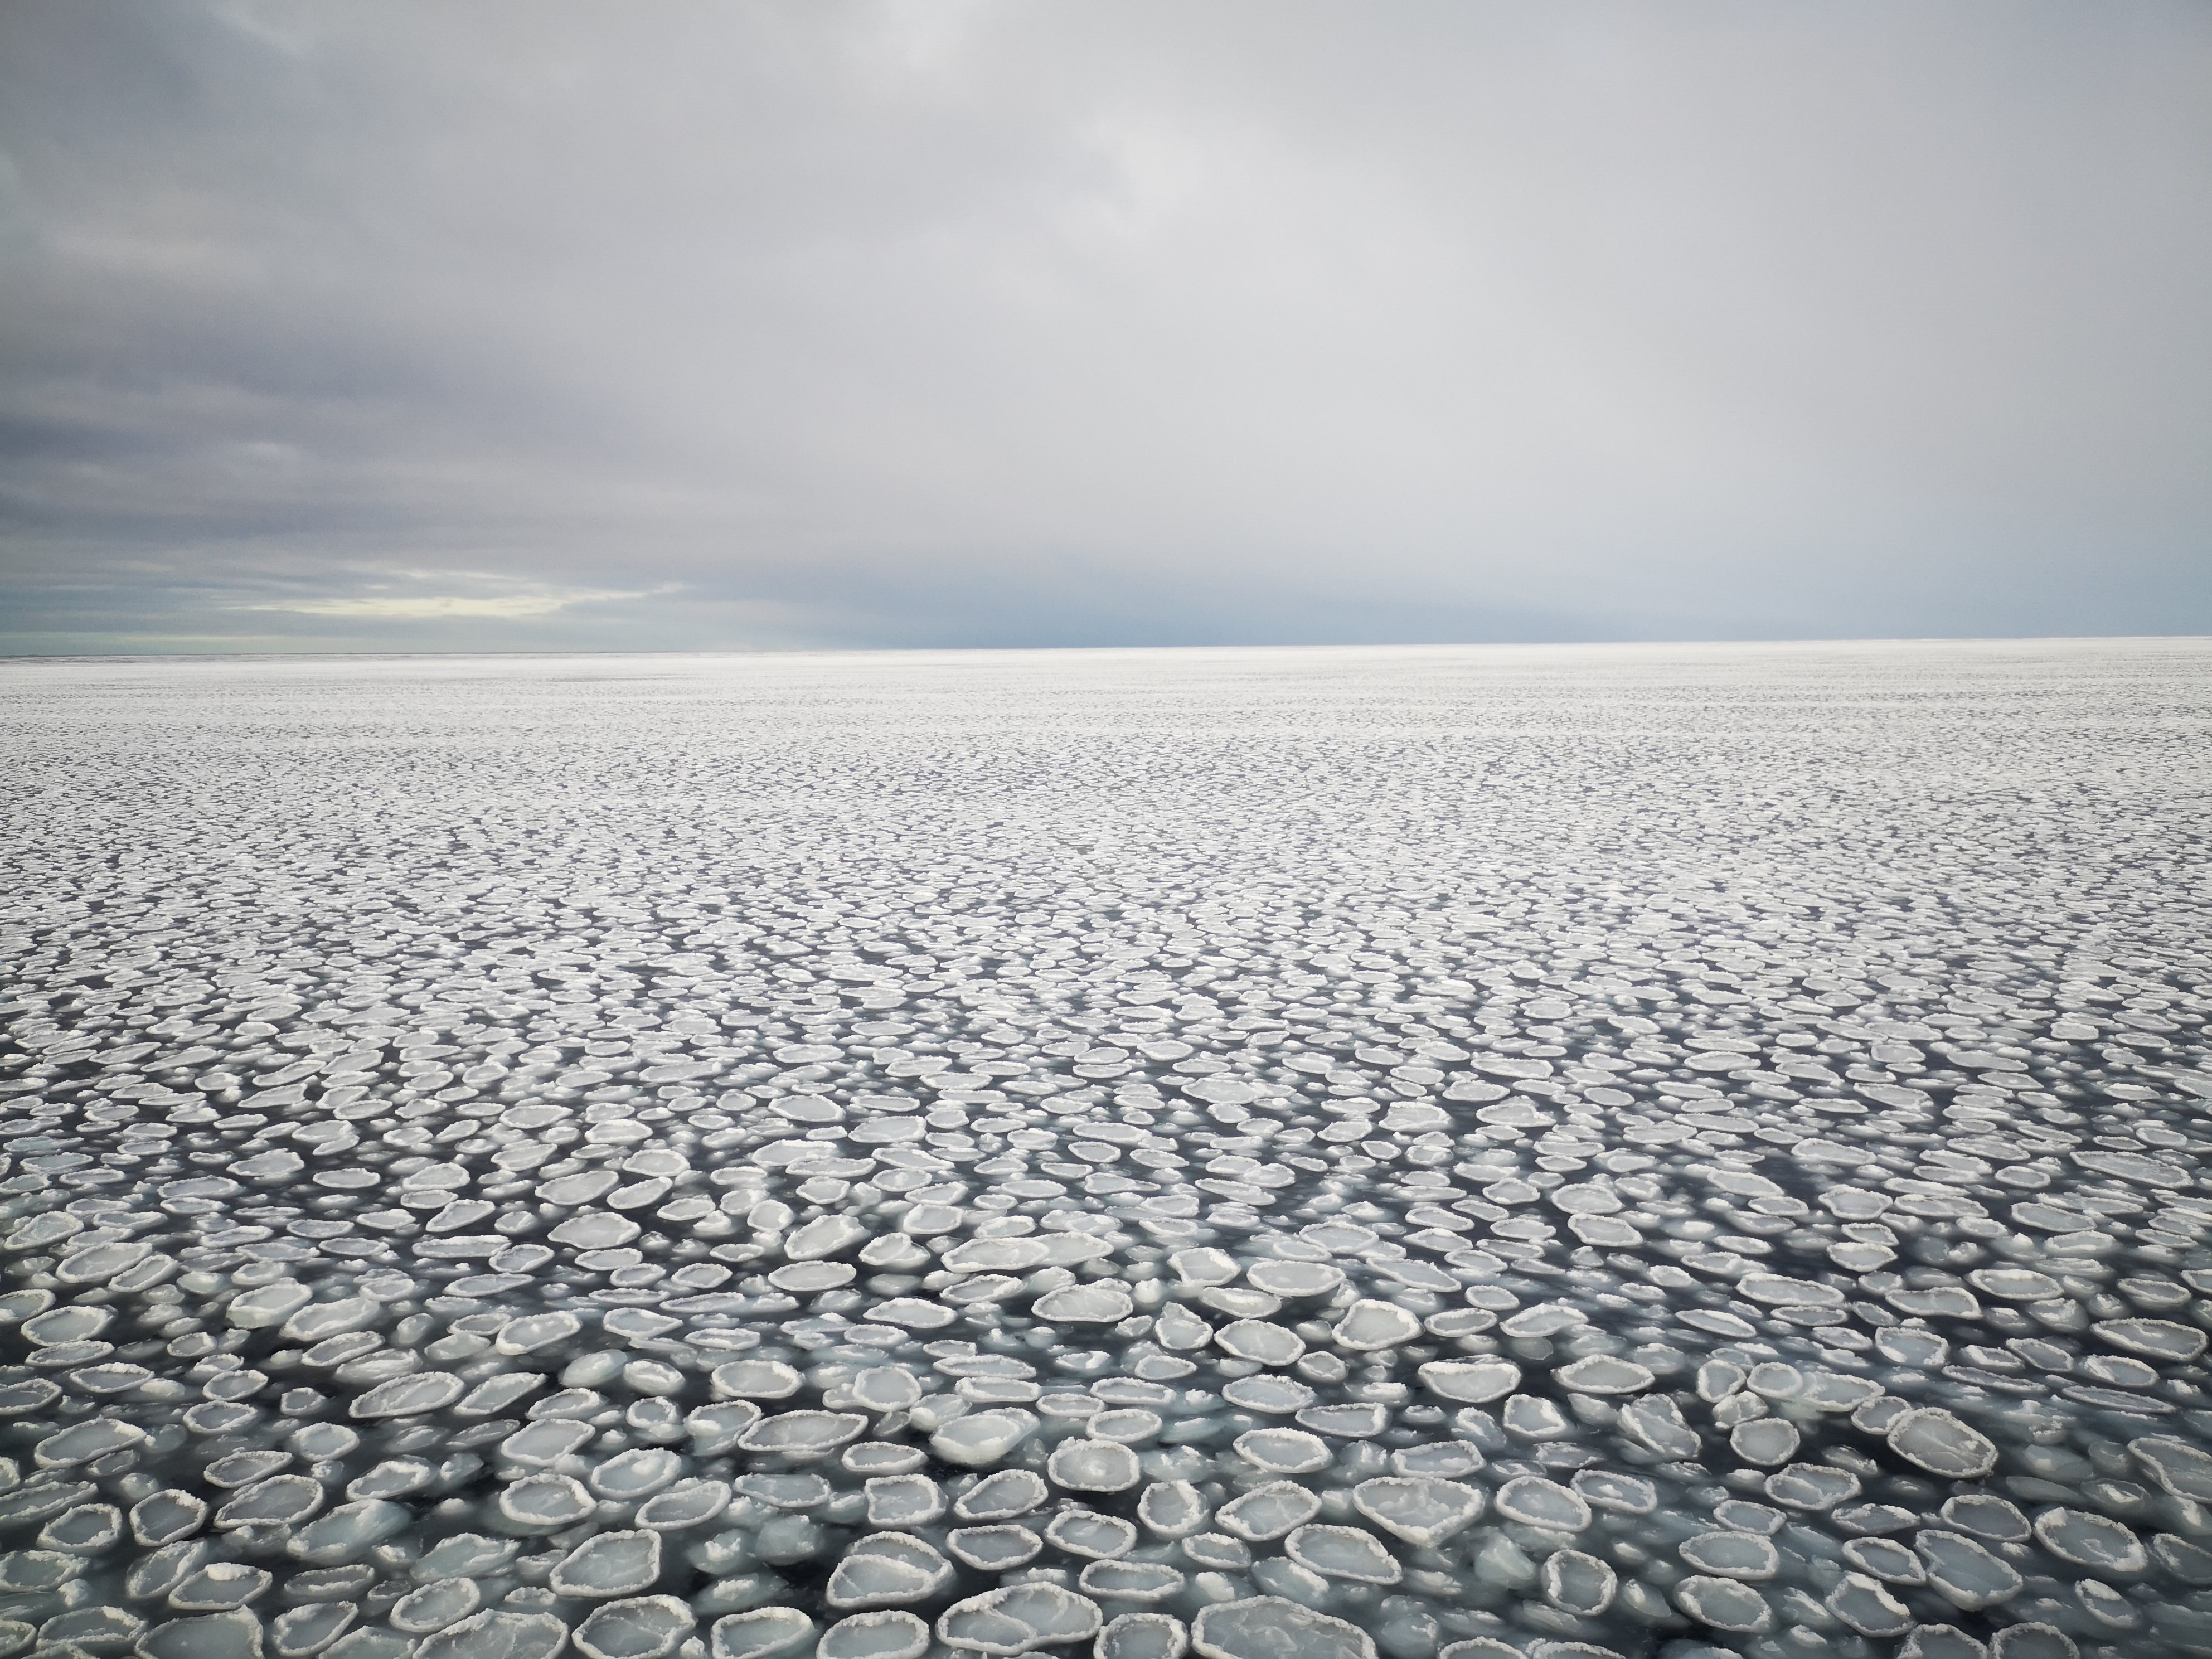
\includegraphics[width = 10cm, height = 6cm]{MIZICE.jpg}
    \caption{Sea ice in the Southern Ocean MIZ during July 2019, where pancake ice is the predominant  concentration while brash ice is the smallest. Swell waves can also be observed propagating through the region Photo taken during SCALE winter cruise July 2019 by the Author.}
    \label{fig:MIZICE}
\end{figure}

Antarctic sea ice has gained recognition for playing a critical role in global climate systems \cite{kennicutt2016delivering}. There has been growing interest by the global scientific community in Antarctic research since the first International Polar Years \cite{kennicutt2016delivering}. International collaborations have sought to formalise Antarctic Research and unite efforts under common goals \cite{kennicutt2016delivering} with the formation of the Scientific Committee on Antarctic Research (SCAR), which has resulted in increased sampling in the MIZ. However, data from the marginal and packed ice zones are under-sampled and poorly represented \cite{vichi2019effects}. Very little in situ data exist to fully understand the environmental conditions surrounding the key metamorphic phases of sea ice in the MIZ. Current climate models and observations exist based on data sets from the Arctic \cite{vichi2019effects} which, when applied to Antarctic sea ice, fail to accurately capture the dynamics of the region on a high-resolution scale. Sea ice expeditions have traditionally taken place during the summer months when the sea ice extent is at a minimum \cite{kennicutt2016delivering}. This results in temporal and spatial gaps in seasonal measurements, which fail to characterise sea ice expanse during the fundamental formation periods \cite{MAKSYM2012seaiceextent}. Additionally, these data are critical for understand Southern Ocean sea ice dynamics and observed phenomenon in the Marginal Ice Zone such as waves-in-ice \cite{kohout2014storm}. Additionally, polar oceanic and atmospheric measurements are critical for understanding the local climates since the high cyclonic activity in the region affects the heat and moisture delivery to higher latitudes. \cite{vichi2019effects}.

Almost all data collected from in situ measurements in the region are taken during seasonal manned expeditions. Only 22 countries have access and shipping capabilities to initiate expeditions to the region. Additionally, these expeditions require vast resources and complex logistical operations. Furthermore these missions are time sensitive and cancelled expeditions create gaps in seasonal data sets. The harsh seasonal climate causes certain, vital areas of the MIZ and packed ice zones to become inaccessible during winter months. As a result, missions only occur during certain seasons resulting in temporal gaps. Attempts have been made to fill in these gaps using data from Arctic climate models, however, these attempts fail to characterise the region and accurately capture seasonal variability. For example, in 2016, an anomaly in the sea ice extent was detected where the ice retreated 48\% faster than the mean rate \cite{turner2017unprecedented}. Furthermore, current climate models do not account for regional discrepancies in Antarctica. \textcite{vichi2019effects} have shown the region to be a hot-spot for cyclonic activity, which regularly impacts ice formation within the marginal ice zone. However these interactions are not captured by current climate models \cite{vichi2019effects}.\par

\begin{figure}[H]
    \centering
    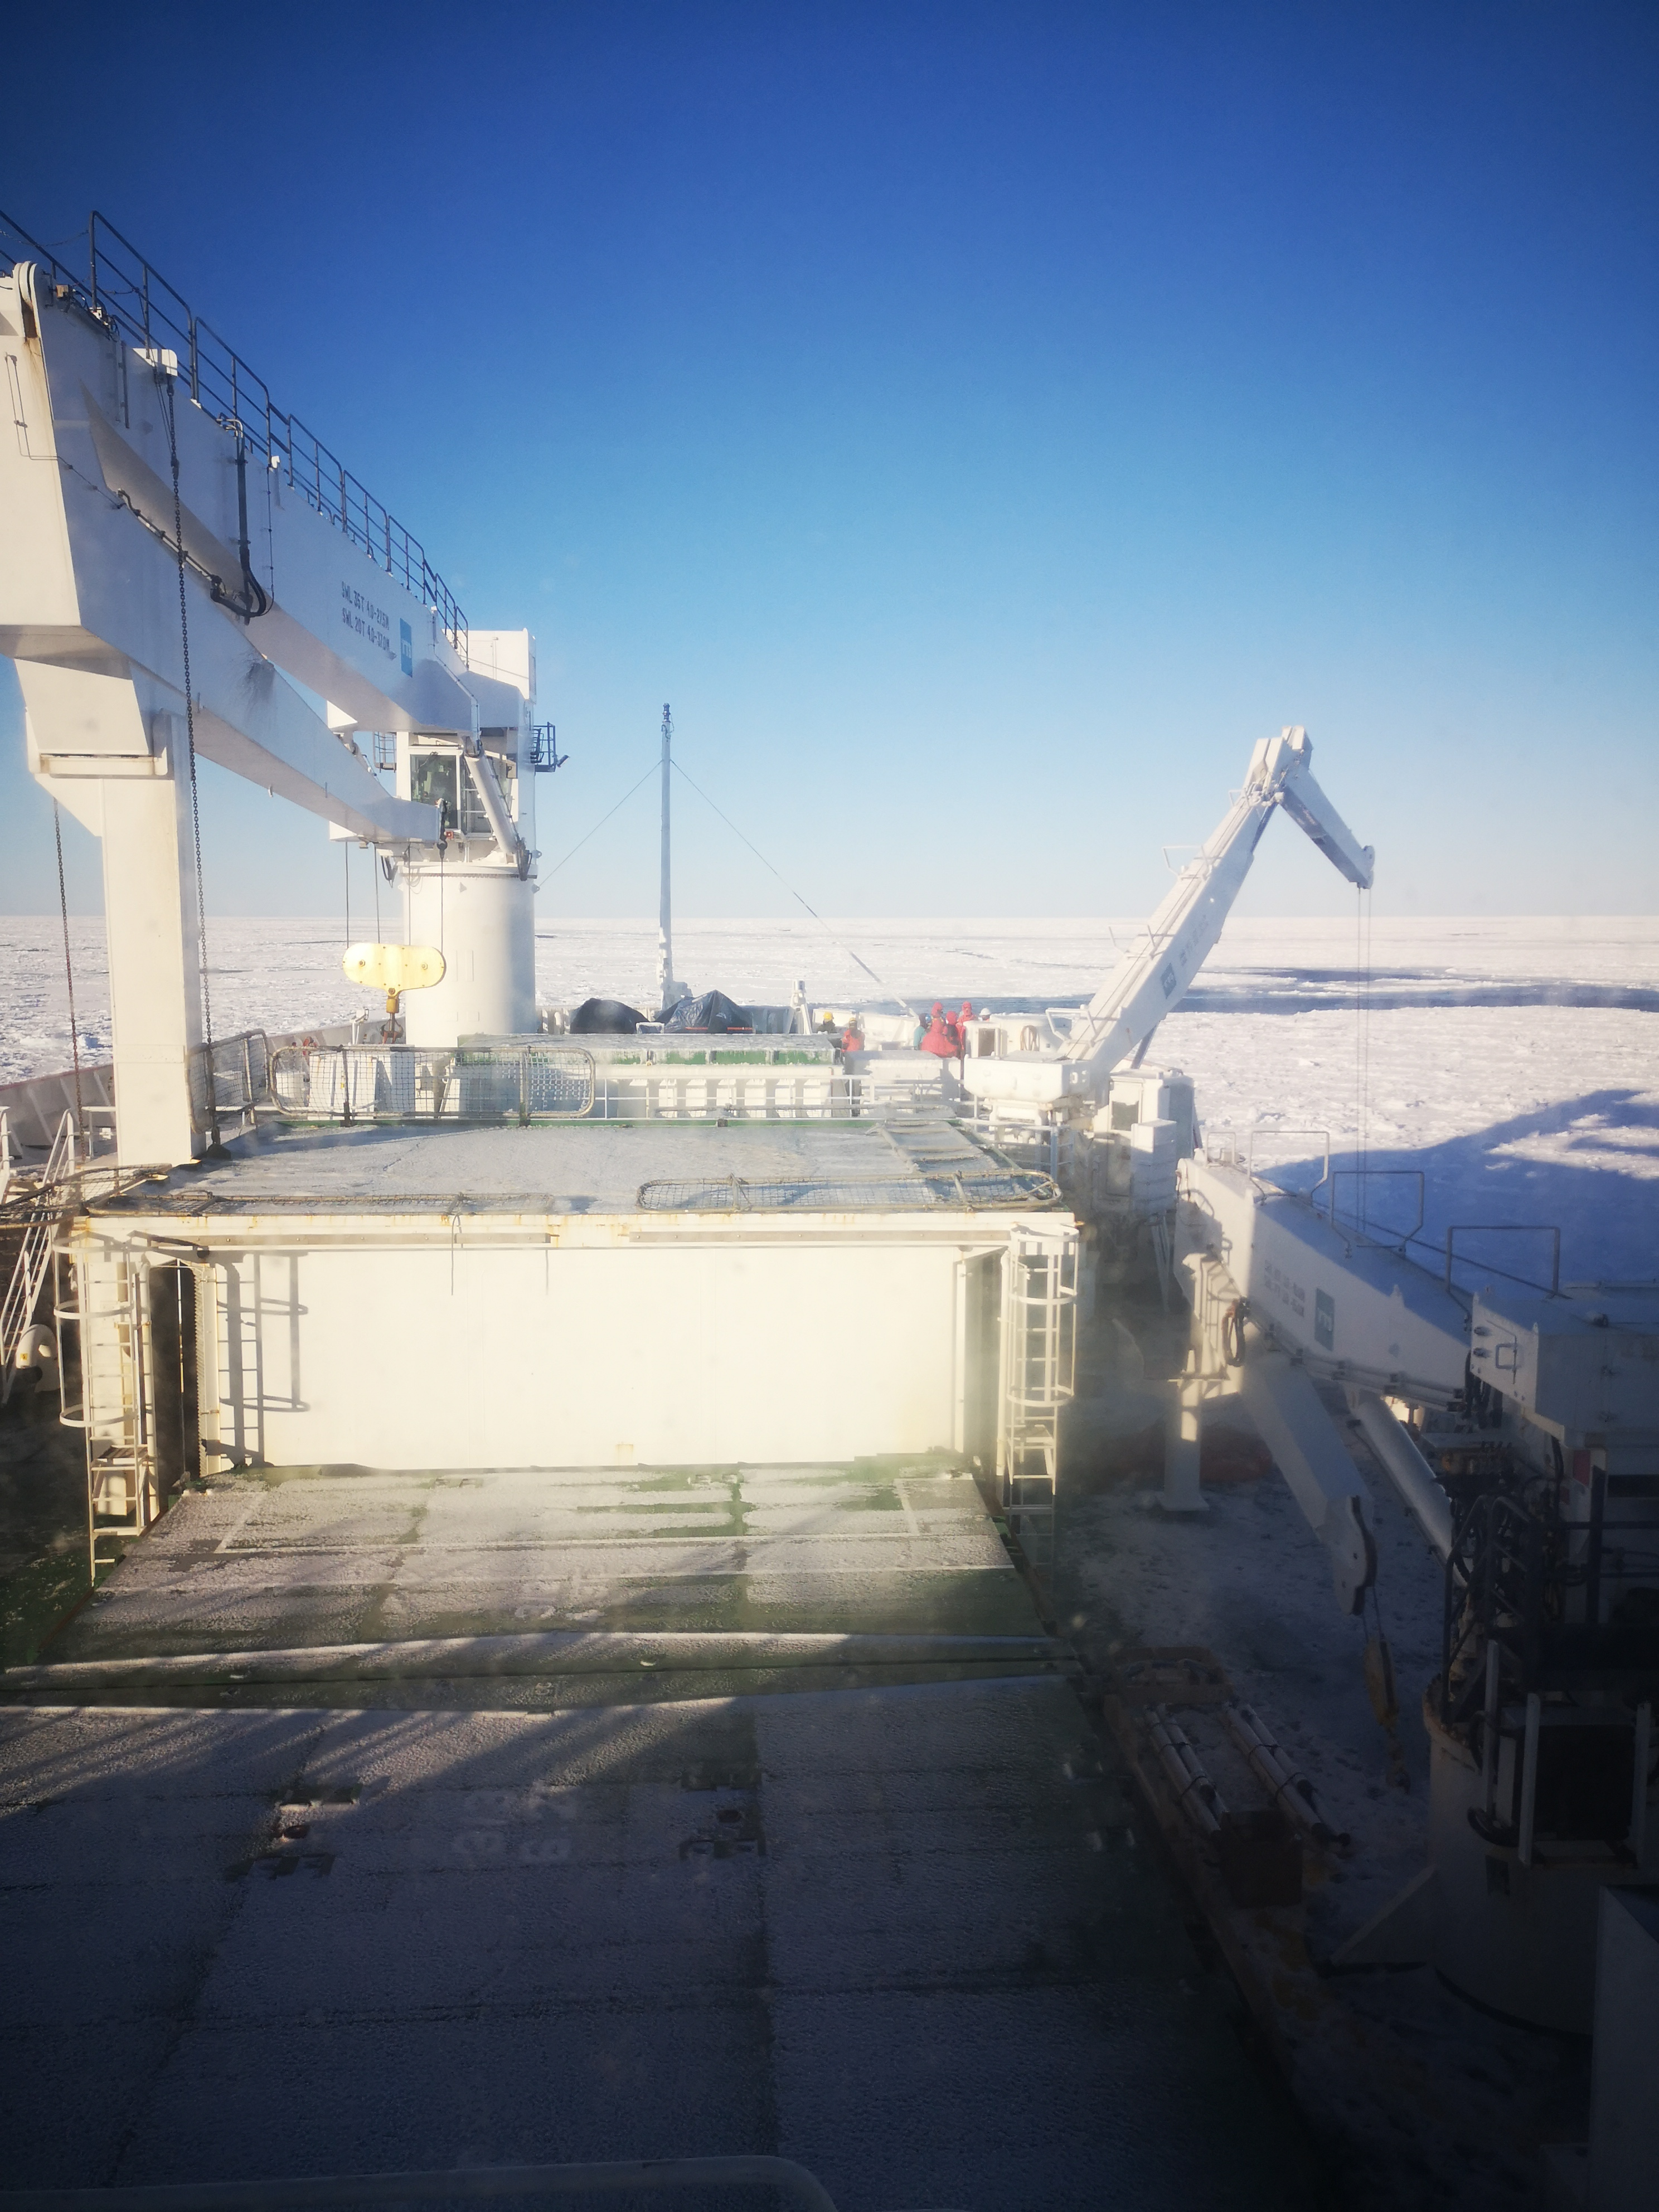
\includegraphics[width = 5cm,height = 7cm]{SHIPACT.jpg}
    \caption{Photo taken in the Marginal Ice Zone from on-board the SA Aghulus II during the SCALE expedition in 2019 by the author.The vessel is anchored in consolidated ice with the UCT \protect\footnotemark -UDE\protect\footnotemark sea ice team performing ice coring activities on the surface of the ice.}
    \label{fig:cruise}
\end{figure}
\footnotetext[2]{University of Cape Town}
\footnotetext[3]{University of Duisburg-Essen}

Therefore, a call to increase sensing in the region has arisen to fill in the gaps of these temporal data sets \cite{kennicutt2019sustained}. A review by \textcite{kennicutt2016delivering} highlights a need to revolutionise Antarctic science to overcome these challenges \cite{kennicutt2016delivering}. As part of the plan, SCAR identified technology as playing a pivotal role in Antarctic research. Air, sea and space-borne technologies can replace manned-expeditions which can provide in situ monitoring on a macro and micro scale \cite{kennicutt2016delivering}. Technology can provide a potential solution to long-term monitoring. Robust, power-efficient solutions that are capable of performing long-term functions in a non-invasive manner are required to reduce the need for implementing new infrastructure.\par

\begin{figure}[H]
    \centering
    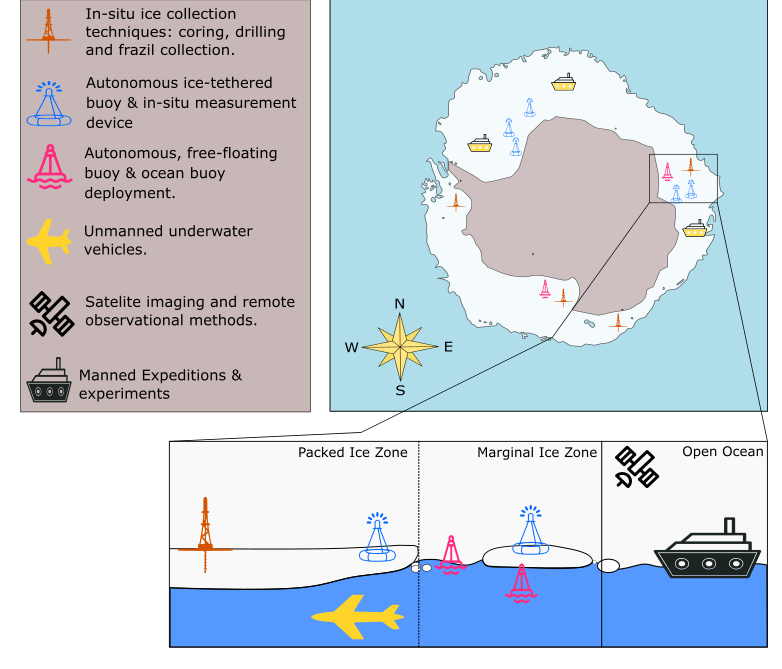
\includegraphics[scale=0.5]{tech.png}
    \caption{ Diagram showing the current state of Antarctic sea ice measurement technologies for each level of observation as well as the estimated deployment location. Diagram taken when sea ice extent is at a maximum. This diagram is derived from the technology implementation strategy identified from the 2016 SCAR roadmap \cite{kennicutt2019sustained}\protect\footnotemark and has been adapted to show sea ice observational techniques. }
    \label{fig:chapter1_tech_diag}
\end{figure}

\footnotetext{Figure made using icons from Flaticon.com, Buoy by hunotika from the Noun Project, oil rig by Mourad Mokrane from the Noun Project, Plane by jokokerto from the Noun Project}

Modern technology has seen an increased use in remote monitoring of the continent \cite{kennicutt2016delivering}. For example, satellite imaging is the most prevalent technology for monitoring sea ice in both the Arctic and Antarctic regions. It provides large-scale mappings of sea ice extent, thickness, snow cover at  the cost of a low spatial resolution \cite{turner2017unprecedented,galin2011validation,alberello2019drift}. Coupling satellite observation with existing climate models allows scientists to extract these parameters from pixels of a satellite image \cite{galin2011validation}. These techniques allowed for the detection of the sea ice retreat recorded in 2016 \cite{turner2017unprecedented} and are very useful for large-scale representation. However, satellite imaging is severely constrained by its resolution \cite{emery1997satellite}. Pixel sizes are in the order of 10 to 100 m \cite{galin2011validation} where, for example, snow thickness can vary down to the cm. Furthermore, cloud cover can compromise the measurements resulting in missing data. Finally, these measurements require validation against data models, which tend to underrepresent climate in the region \cite{galin2011validation,emery1997satellite}. Hence, a need arises for the development of in-situ technology that can provide accurate, detailed information down to the highest possible resolution and allow for long term, large scale monitoring of ocean-ice-atmosphere processes. Hence we turn to autonomous platforms as a solution.\par 
\begin{figure}[H]
    \centering
    \begin{subfigure}[t]{.3\textwidth}
    \begin{tikzpicture}
    \node[anchor=south west,inner sep=0] (image) at (0,0) { 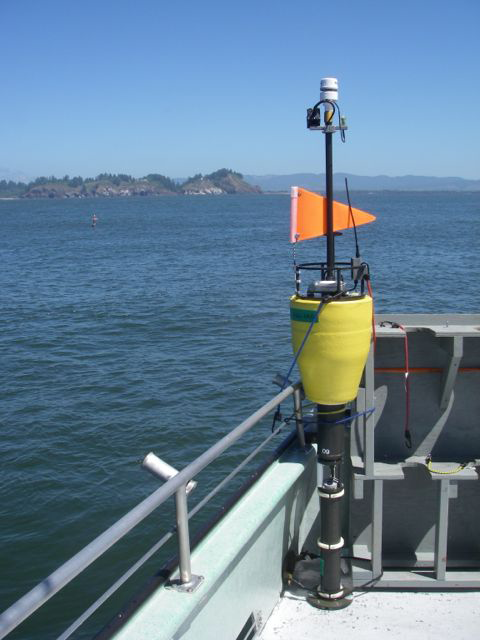
\includegraphics[width = 4cm, height = 6cm]{swift_4.png}};
    \begin{scope}[x={(image.south east)},y={(image.north west)}]
        \draw[color=black, ultra thin,fill=white] (0.0,0.0) rectangle (0.21,0.16) node[pos=.5] {A};
    \end{scope}
    \end{tikzpicture}
    \end{subfigure}
    \hfill
    \begin{subfigure}[t]{.3\textwidth}
        \begin{tikzpicture}
    \node[anchor=south west,inner sep=0] (image) at (0,0) {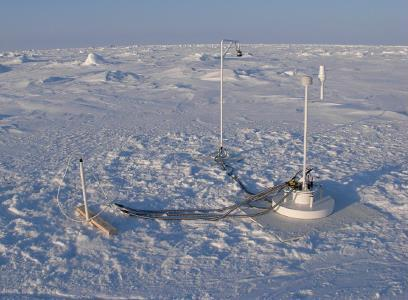
\includegraphics[width = 4cm, height = 6cm]{IMBBuoy1.jpg}};
    \begin{scope}[x={(image.south east)},y={(image.north west)}]
        \draw[color=black, ultra thin,fill=white] (0.0,0.0) rectangle (0.21,0.16) node[pos=.5] {B};
    \end{scope}
    \end{tikzpicture}
    \end{subfigure}
    \hfill
     \begin{subfigure}[t]{.3\textwidth}
      \begin{tikzpicture}
    \node[anchor=south west,inner sep=0] (image) at (0,0) {        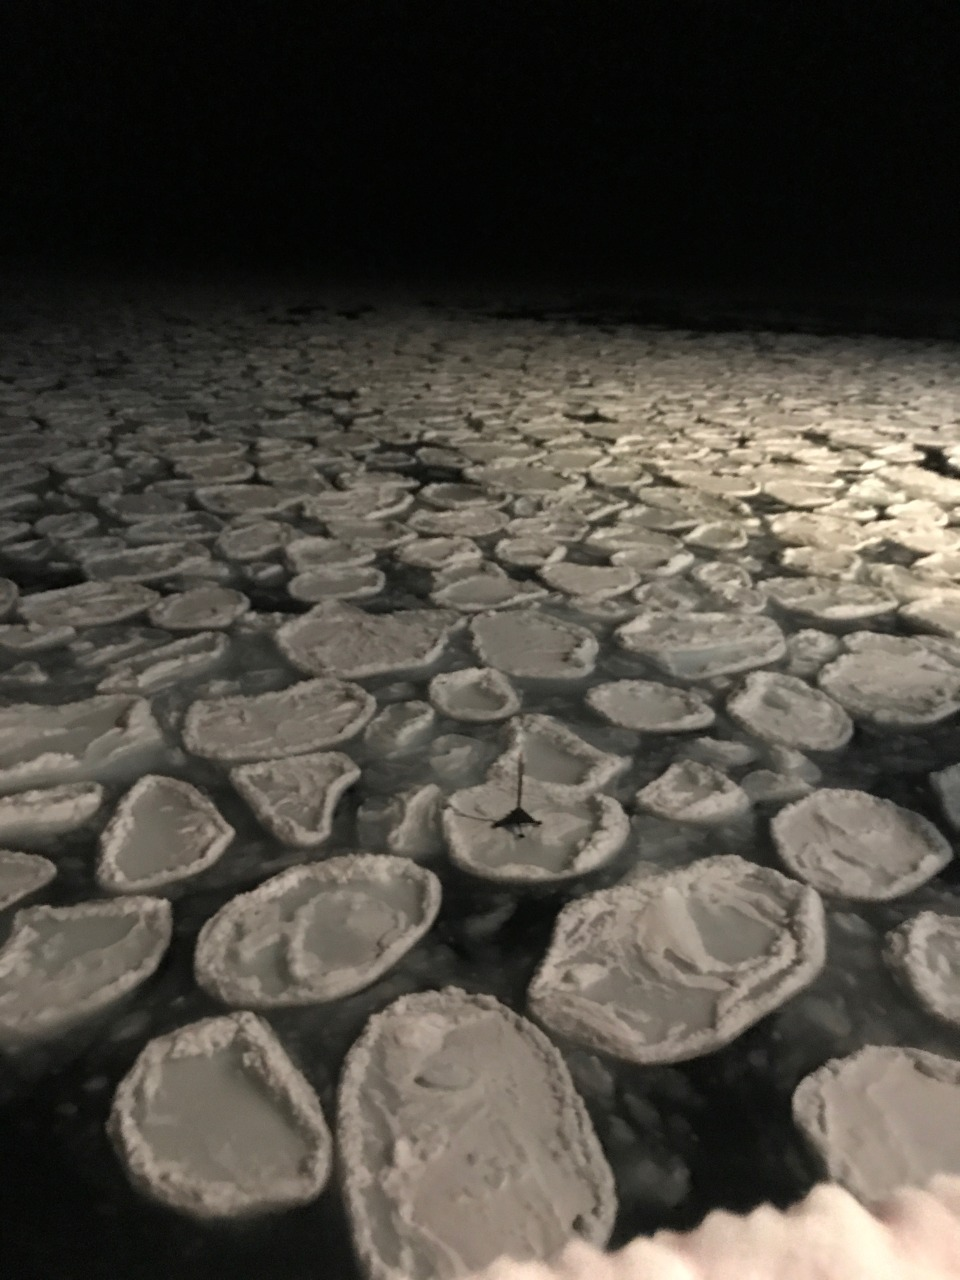
\includegraphics[width = 4cm, height = 6cm]{deploy.jpg}};
    \begin{scope}[x={(image.south east)},y={(image.north west)}]
        \draw[color=black, ultra thin,fill=white] (0.0,0.0) rectangle (0.21,0.16) node[pos=.5] {C};
    \end{scope}
    \end{tikzpicture}
    \end{subfigure}
    \hfill
    \caption{Practical examples of instruments used to collect in situ measurements in the sea ice region. These comprise: (A) the Surface Wave Instrument
Float Tracking (SWIFT) buoy developed by the University of Washington [\cite{thomson2012wave} image source:\cite{swift}]; (B) the Ice Mass Balance (IMB) buoy developed by Dartmouth College [\cite{PLANCK2019102792} image source: \cite{simbfact}]; and (C) the Southern Hemisphere Antarctic Research Collaborative (SHARC) buoy developed by the University of Cape Town (photo courtesy of Robyn Verrinder).}
    \label{fig:chapter1_prac_buoys}
\end{figure}

Delivering a remote system capable of long-term functionality is a high priority for Antarctic science \cite{kennicutt2016delivering} and will accrue robust, reliable, time-sensitive data-sets to populate these models. This will bring climate models in line with current observations and will allow for a quantified, thorough description of a local phenomenon, for example, the role of ocean swells in ice formation in the Marginal Ice Zone \cite{doble2013wave}. A successful system should have the following characteristics: \footnote{Taken from a collective survey distributed during the Antarctic Roadmap Challenge in 2016 \cite{kennicutt2016delivering}} 
\begin{enumerate}

    \item Autonomous or sustained deployment capabilities
    \item Adequate remote sensing capabilities
    \item Improved, robust power supplies
    \item Real-time data collection, transfer and analysis
    \item Survivable under extreme weather conditions
\end{enumerate}

However, the current state of  modern Antarctic observational technology is underdeveloped; current prototypes are too expensive and difficult to obtain by the scientific community \cite{kennicutt2016delivering}. Many institutions have initiated projects to develop autonomous systems such as buoys (examples shown in figure \ref{fig:chapter1_prac_buoys}) and unmanned surface vehicles (USVs) such as Wave Gliders \cite{liquidrobot2016wave,swart2020submesoscale}. These devices have been utilised successfully in Antarctic and Arctic oceanographic studies. For example, SWIFT buoys deployed in the Antarctic Marginal Ice Zone was used to quantify ice floe sizes in the region \cite{alberello2019brief}. However, these systems are extremely niche and require a technical crew to deploy and retrieve the buoys. The devices are generally proprietary with fixed sets of sensors and fewer sensing capabilities rendering the device inflexible to the needs of scientists \cite{rabault2017measurements}. \textcite{rabault2019open} note the growing use of open source hardware and off-the-shelf technology in modern systems. Off-the-shelf  components have reached a state where the components are well documented and well specified to withstand the requirements for polar systems \cite{rabault2019open}. Open-source hardware has allowed for the free exchanging of designs allowing scientists to build their own devices without needing to design and test prototypes \cite{rabault2019open}. As a result, there has been a growth in literature on open access devices with designs and code bases readily available on code sharing sites such as GitHub\footnote{For example: see \textcite{rabault2019open} Github repository at \url{https://github.com/jerabaul29/LoggerWavesInIce_InSituWithIridium}}Hence, inclusion of cost-effective technology as a solution is a growing trend. \par 

Additionally, these devices have shown promise in the field. \textcite{rabault2019open} developed an open-source multi-sensing autonomous system and \textcite{kohout2015device} developed a multi-sensing system with off-the components. The devices were deployed in the Arctic and Antarctic Marginal Ice Zones. The buoys developed by \textcite{kohout2015device} encountered technical issues resulting in a total of 39 days survivability with two buoys lost immediately after deployment, one buoy surviving for nine days and another for 17.5 days \cite{kohout2015device}. The buoys developed by \textcite{rabault2019open}  included solar panels to recharge the batteries. However these systems survived for only 12 days during the spring.  Other systems deployed in the region are the MetOcean buoys \cite{uptempo}, Surface Wave Instrument Float Tracking (SWIFT) \cite{thomson2012wave} buoys and Trident buoys \cite{trident}. These systems, however, are expensive and do not have the sensing capabilities specifically for sea ice dynamics. Consequently, this presents a problem for in situ sea ice observations in that multiple systems are required to collect desired data for models with a need for back up systems in case of failure. 

Therefore we are presented with a unique opportunity to design a series of novel ice-tethered autonomous systems to increase remote sensing at an affordable rate. The goal of the project is to design a proof of concept system with expandable, modular capabilities capable of running off a single power module for seasonal periods. This project will form part of a larger research effort lead by the joint University of Cape Town (UCT) and University of Duisberg-Essen (UDE) Sea Ice research team. The focus of this collaboration is to better understand sea ice lifecycle in the Southern Ocean. Hence, the proposed system aims to provide a low cost, easy to deploy environmental data measurement system that can be expandable to operate in a network allowing for a single-system deployment strategy. In this thesis, the firmware design of a novel ice-tethered buoy for the Antarctic Marginal Ice Zone is presented. The goal is to develop a robust software system  for a platform built using off-the-shelf components to monitor ice drift, atmospheric conditions and waves-in-ice measurements over a full seasonal cycle.

\begin{figure}[H]
    \centering
    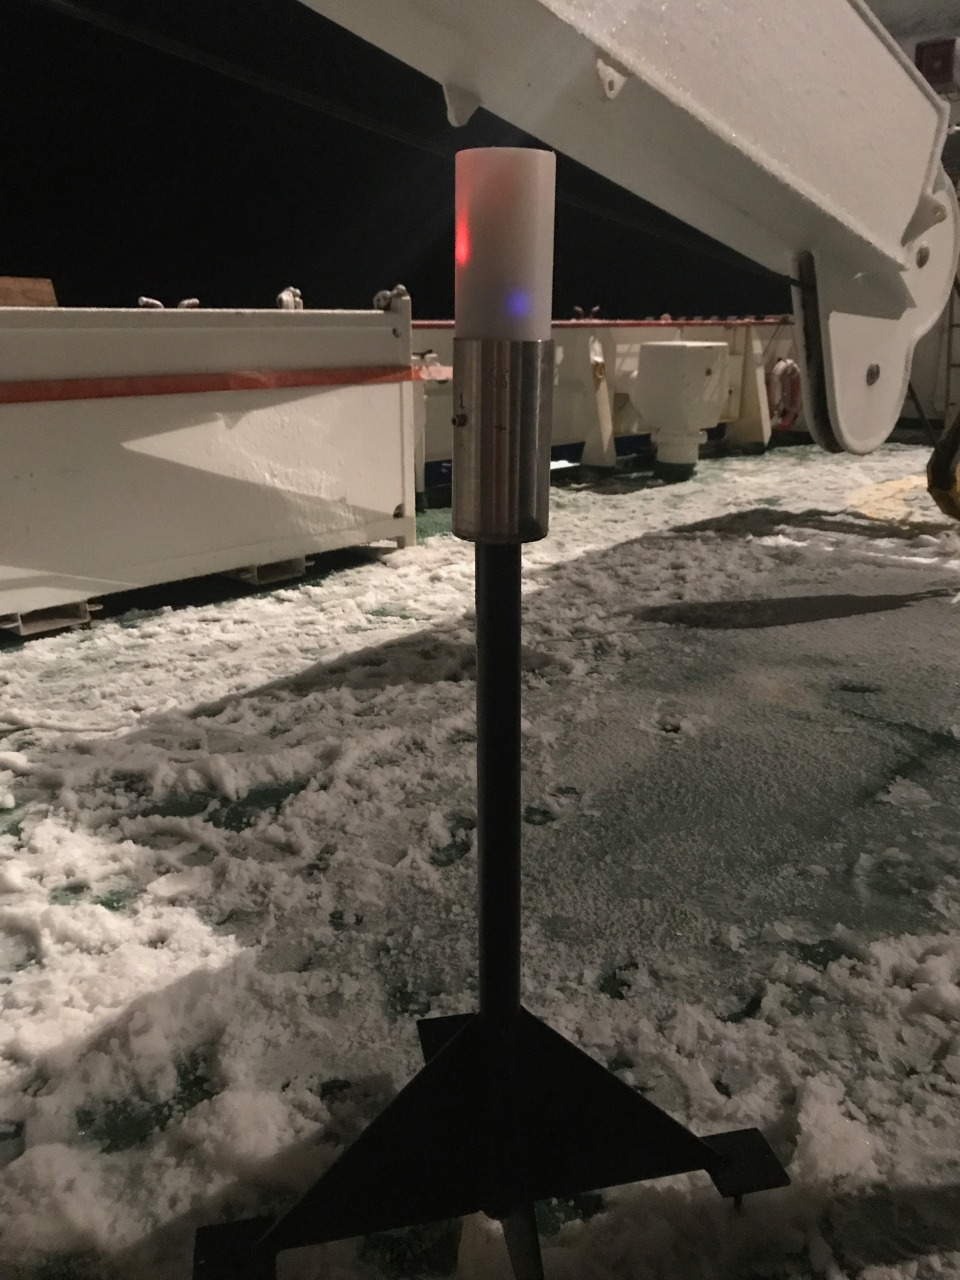
\includegraphics[width = 6cm, height = 8cm]{SHARC.jpeg}
    \caption{Novel Ice drift, environmental monitoring and wave measurement autonomous platform: the Southern Hemisphere Antarctic Research Collaboration (SHARC) Buoy.Developed by the University of Cape Town. Photo by R. Verrinder.}
    \label{fig:chapter1_sharc_buoy}
\end{figure}


%====================================================
\section{Problem statement}
\label{subsec:ch1.section2}

This project aims to design a prototype system to monitor environmental conditions that lead to the formation of ice floes in the Marginal Ice Zone. The goal of the project will be to increase remote sensing in an affordable manor while allowing for easy access to the technology and data.  Conclusion of this project will result in a fully automated system that can be deployed on an ice floe in various locations in the Marginal Ice Zone up to the Packed Ice Boundary Layer. Transfer of data from the system will occur using the available infrastructure in the region to reduce costs and make the system as non-invasive as possible. Furthermore, the resulting system will run off a portable power source with limited charging capability to survive for at least one month. By identifying and engaging with key stakeholders in the project, we aim to design a system using off-the-shelf components and synthesize components into a low-cost, high-performance solution with the final deliverable being a deployable system for the Next South African Antarctic expedition to the Marginal Ice Zone.  Thereby creating the following project objectives:
\begin{enumerate}
    \item Perform a literature review of the current state of remote sensing in the Southern Ocean, analysing the techniques and strategies implemented by each system.
    
    \item Engage with key stakeholders to create a set of user requirements for the system, translate these requirements into system specifications, identifying critical subsystems and synthesising them into a high-level system.
    
    \item Identify a suitable network for remote communication as well as the corresponding communication module.
    
    \item Select suitable hardware components and develop a robust set of libraries and unit tests for each system.
    
    \item Identify the energy requirements and select a suitable power source.
    
    \item Identify a processor/set of processors that meet the requirements for the system and develop firmware in C using a Hardware Abstract Layer (HAL).
    
    \item Connect the subsystems to a motherboard and place the system in an enclosure capable of protecting the system from the harsh climate.
     
    \item Evaluate the platform against a serious of unit tests, robustness tests and  hardware tests.
    
    \item Deploy the system in the Marginal Ice Zone and monitor performance.
\end{enumerate}

%----------------------------------------------------

%====================================================

\subsection{Project Initiation}

The project was initiated in 2018 with input from the following stakeholders.
\begin{table}[H]
    \centering
    \caption{legend showing the key stakeholders in the initiation of the project as discussed in the phases below. Legend includes name, reference number and department/institution. }
    \label{tab:proj_init_members}
    \begin{tabular}{||c|l|l|l||}
    \hline
        \textbf{Reference:} & \textbf{Name:} & \textbf{Institution} & \textbf{Department}  \\
        \hline
        1 & Jarryd Son & University of Cape Town & Electrical Engineering \\
        \hline
        2 & Nadir Vorajee & University of Cape Town & Electrical Engineering \\
        \hline
        3 & Prof Amit Mishra & University of Cape Town & Electrical Engineering \\
        \hline
        4 & A/Prof Marcello Vichi & University of Cape Town & Oceanography \\
        \hline
        5 & A/Prof Sebastian Skatulla & University of Cape Town & Civil Engineering\\
        \hline
        6 & Marc de Vos & South African Weather Service & N/A \\
        \hline
    \end{tabular}

\end{table}

\subsubsection{Concept phase}

The concept design was performed by Son and Vorajee (1,2) under the supervision of Prof Mishra (3). The design was presented at the first meeting on the 11 September 2018 with principle stakeholder A/Prof Vichi (4) and A/Prof Sebastian Skatulla (5). The proposed device was presented as an upgraded version of the Trident sensing buoy with expanded sensing capabilities. During the meeting, it was agreed to deploy and test the system during the Winter and Spring SCALE expeditions in 2019. The provisional dates for these cruises were: July 2019 and November 2019 respectively. A follow up meeting occurred on the 4th October 2018 where de Vos (6), (South African Weather Service (SAWS)) expressed interest in the research and the development of the project. de Vos (6) provided additional context for the project and presented current work conducted by SAWS.

\subsubsection{Procurement phase}

A preliminary user requirement was conducted by Son and Vorajee (1, 2). From there, suitable components for each of the subsystems were selected with orders being placed on the 19th December 2018. This order included sensors, a GPS, short range communication modules (Xbees), satellite communication modules (Iridium), STM32F1 micro-controller and IMUs.

\subsubsection{Handover phase}

The project was handed over to Jamie Jacobson under the supervision of Robyn Verrinder on the 8th February 2019, officially commencing the prototyping phase of the project.
%----------------------------------------------------

%====================================================
\subsection{Scope}

This project will focus on the firmware design for the buoys. The outcome of this study will be a robust set of firmware and unit tests to validate the firmware against. The project timeline will take place from February 2019 to December 2020 with key deliverable dates being:

\begin{enumerate}
    \item 18 June 2019 - SCALE Winter Cruise  (Version 1.0 Complete)
    \item 12 October 2019 - SCALE Spring Cruise (Version 1.0 Revisions)
\end{enumerate}

Final submission is expected to take place in February 2021 with a departmental paper written by March 2021. \par 


The project will hence focus on the software development of the project. Hardware design will not be included in this study and future designs will be discussed as recommendations. This includes the mechanical structure and the electronic modules. However, this project will include the selection of devices, which will be evaluated against the technical specifications. Additionally, the hardware modules will be described.\par 

System testing will be conducted on a subsystem software level and a full system. The testing procedures are described in Sections  \ref{tab:AT001} to \ref{tab:AT009}. 

Large scale calibrations will not be included in the project scope due to tight timeline constraints. Finally, the  design, implementation and calibration of an IMU-based wave measurement algorithm will not be explored in this project. The IMU however, will be validated and verified by sampling enough data to fit into a single Iridium transmission packet. 
%----------------------------------------------------

\subsection{Limitations and constraints}

The largest limitation to the project will be the time constraints. The project timeline coincides with the SCALE Research cruise using the winter and spring expeditions for buoy deployment thereby limiting the time frame for development. Additionally, the firmware development will be limited to the capabilities of selected processor. \par 

The firmware development is heavily constrained by the hardware selected for the platform. Peripheral drivers were written for modules that were agreed upon by the project members. Additionally, the IMU, processor, environmental sensor and satellite modem components were pre-selected in 2018. The firmware was thus constrained by design choices originally made in 2018 and early 2019 for the first version of the system however, these designs were revised for subsequent versions of the buoy from September 2019. As a result of the time constraints and hardware constraints, the devices were designed without previous knowledge of the environment and with a limited number of sensors.  Finally, the selected processor has a limited number of communication peripherals which influenced the type of sensor that was selected. Firmware was therefore constrained to the hardware configuration of the module.

The communications network in Antarctica is severely limited and the most reliable form of remote communications is the Iridium Satellite Network. The amount of data that can be transmitted is severely limited by the satellite network in terms of bandwidth, data costs, packets structure and reliability of transmission. Testing for Antarctic conditions is severely limited by available testing facilities, therefore, rigorous environmental tests may only be conducted during the expeditions.\par 

The first prototype was deployed with a limited number of sensors due to the development constraints. Mechanical failures resulted in the buoys ceasing operation within an hour of deployment. Further development occurred in 2020 to increase the sensing capability of the buoy however due to the 2020 COVID 19 outbreak, all expeditions were canceled for the year therefore final system testing in Antarctica was not possible. Attempts were made to deploy the devices on other expeditions from other countries however, shipping delays were encountered preventing the device from reaching the expedition team on time. Currently, a prototype version has been sent onboard the SA Agulhas II to the SANAE IV base on the continent where testing is expected to take place in late February 2021. This falls outside the time frame of this dissertation. Instead, the buoy will be tested on the home  continent with low temperature tests being conducted in a commercial $-20\degree \text{C}$ Freezer. Future deployment arrangements are currently being made with a German Expedition onboard the RV Polarstern which will begin early to mid 2021.

\subsection{Assumptions}

The device has sufficient power to access any of the sub modules if required. Devices that pass a connection test, are considered "online" and capable of producing reliable data. The processors are the ARM-based  STM32L4 and STM32F4 microcontrollers and do not come preloaded with any real time/operating system. Development will take place using the Hardware Abstract Layer (HAL) driver files and all hardware that has been selected is rated for the environmental conditions described in Section \ref{sec:ch1.section1}. A system/subsystem is considered valid if it passes a suite of acceptance tests and verified if it meets the functional requirements. Devices that are not active need to be placed in power down mode. Finally, the system is considered complete if it can complete a single measurement cycle from power on without the assistance of any auxiliary equipment.
%----------------------------------------------------

%====================================================
\section{Plan of development}
\label{sec:ch1.section3}

The plan of development describes how the project was conducted through the various stages. A literature review was conducted to analyse the current state of Antarctic climate modeling and the state of technology in the region. Then, a problem statement was defined by engaging with project stake holders and developing a set of user requirements. The user requirements were used to formulate acceptance tests and technical specifications which were used to guide subsystem design and selection. Then, the firmware stage was initiated with the development of API libraries for each module of the device. These were then synthesised and sequenced into a software system defined by short periods of activity and long periods of inactivity. This was used to optimise the device for low power consumption. The system was tested by performing a power consumption test, which was used to evaluate the power characteristics. The device was set outside to run a full transmission cycle. Finally the results were analysed and used to validate the buoy as a viable tool for remote Antarctic monitoring.
\pagebreak
%====================================================
\section{Report structure}
%----------------------------------------------------

\begin{center}
   {\setlength{\extrarowheight}{5pt}%
    \begin{longtable}[H]{|>{\RaggedRight}m{0.15\textwidth}| >{\centering}m{0.2\textwidth} | 
   m{0.65\textwidth}|}
        \caption{Description of report structure including key phases of the project and
        significance}
        \label{tab:report_structure}\\
        \hline
        \textbf{Chapter} & \textbf{Phase} & \textbf{Description} \\
        \hline
        Chapter \ref{ch:chapter2} & Literature review & Description of the state of Antarctic climate modeling is discussed, including stochastic modeling processes and current sampling techniques using un-manned instrumentation. From this review, the key measurands are identified and an analysis of the state of the art will be used to identify the usefulness and areas where SHARC Buoy can provide a solution. \\
        \hline
        Chapter \ref{sec:ch3_design} to \ref{sec:ch3_FR} & System development &  An analysis of project stakeholders is provided as well as an assessment of their needs. Then, a set of user requirements is developed and ranked in order of importance.The functional requirements selected will guide the device selection and, ultimately, be used to evaluate the performance of the final system. This lead to the identification of the critical subsystems shown in table \ref{tab:subsys} and a final system topology choice. A set of technical specifications were derived for subsystem hardware selection and a suite of acceptance tests were written to ensure the components conformed to the desired specifications.\\
        \hline
        Chapter \ref{sec:ch3_sysoverview} to \ref{sec:ch3_final_assembly} & Platform overview & Description of the mechanical and electronic components that were selected for the device. The specifications of each component and price are given. The final system consists of a Ublox Neo-7M GPS, Rockblock 9603 Iridium modem, environmental sensor (BMP280), MPU6050 Inertial Measurement Unit and INA219 power monitor. Flash chips were selected as a permanent storage solution for data during phases of inactivity. The components were synthesised on a stack of three PCBs shown in Figure \ref{fig:top_elec}. A separate power module is shown in Figure \ref{fig:bot_elec}. An overview on the assembly of the project is given to close the section.\\
        \hline
        Chapter \ref{sec:ch3_soft} & Software overview & A complete overview of the software design process is provided. The key features and focus of the software are outlined along with the firmware structure as shown in Figure \ref{fig:soft_arch}. The project structure includes a breakdown of files, structure and driver files. The configuration of the processor for this application is shown as well as various peripherals and configurations used to set the device up for execution. Then a brief discussion about power mode and system selection ensued to provide clarity on the power-consumption optimisation process. Then a description of the firmware is given. A decision was made to implement a state machine. Here, a finite set of routines were defined and a description of the sequencing was given. Finally an over view of the flow of data from the device to the user was provided.\\
        \hline
        Chapter \ref{sec:ch4_systests} to \ref{sec:ch4_remotedeployment} & Testing & In this section, the tests conducted on the platform and the system are given. These include subsystem acceptance test, full system tests, power tests and preliminary deployment test results from the 2019 SCALE winter expedition.\\
        \hline
        Chapter \ref{sec:ch4_final_eval} & Final evaluation & The results of subsystem acceptance tests are used to validate the system. The outcome of the project is compared to the functional requirements to determine the system's performance and verify that the project goals have been met.\\
        \hline
        Chapter \ref{sec:ch4_disc} & Discussion & This section provides a discussion of the results and key findings. The discussion focuses on the limitations of the power module and the outcome of the power test. Additionally, the performance of the device during the deployment test is discussed. An in-depth analysis of additional subsystem limitations is provided along with the performance of the firmware in spite of these limitations. The section concludes with a comparison of the buoy against other devices in the field.\\
        \hline
        Chapter \ref{ch:conclusion} & Conclusion &  The outcome of the project is presented and a conclusion is made about the project outcomes, goals and whether the firmware was able to achieve them.\\[5pt]
        \hline
        Chapter \ref{ch:recommendations} & Recommendations & Improvements and recommendations are provided for future work on the project. These include tests that could not be conducted, research and focus areas as well as hardware/ software improvements. \\
        \hline
    \end{longtable}}

\end{center}
    
%****************************************************
% END
%****************************************************
